\documentclass[runningheads,a4paper]{llncs}

\usepackage[latin1]{inputenc}
\usepackage{graphicx,color,url}
\usepackage[dvips]{epsfig}
\usepackage{verbatim}
\usepackage{tikz}
\usetikzlibrary{shapes,arrows}
\usetikzlibrary{calc,patterns,snakes,decorations.pathmorphing,decorations.markings}
\usetikzlibrary{positioning}
\usepackage{amsmath}

\usepackage{tabularx} % better tables
\usepackage{float}
\setlength{\extrarowheight}{3pt} % increase table row height
\newcommand{\tableheadline}[1]{\multicolumn{1}{c}{\spacedlowsmallcaps{#1}}}
\newcommand{\myfloatalign}{\centering} % to be used with each float for alignment
\usepackage{caption}
\captionsetup{font=small} % format=hang,
\usepackage{subfig}
\usepackage[ruled]{algorithm2e}
%\providecommand{\tabularnewline}{\\}
\usepackage{listings}
\usepackage{color}
\usepackage{graphicx}
\newcommand{\keywords}[1]{\par\addvspace\baselineskip
	\noindent\keywordname\enspace\ignorespaces#1}

\definecolor{dkgreen}{rgb}{0,0.6,0}
\definecolor{gray}{rgb}{0.5,0.5,0.5}
\definecolor{mauve}{rgb}{0.58,0,0.82}
\definecolor{gray}{rgb}{0.4,0.4,0.4}
\definecolor{darkblue}{rgb}{0.0,0.0,0.6}
\definecolor{lightblue}{rgb}{0.0,0.0,0.9}
\definecolor{cyan}{rgb}{0.0,0.6,0.6}
\definecolor{darkred}{rgb}{0.6,0.0,0.0}


\lstset{
	basicstyle=\ttfamily\footnotesize,
	columns=fullflexible,
	showstringspaces=false,
	numbers=left,                   % where to put the line-numbers
	numberstyle=\tiny\color{gray},  % the style that is used for the line-numbers
	stepnumber=1,
	numbersep=5pt,                  % how far the line-numbers are from the code
	backgroundcolor=\color{white},      % choose the background color. You must add \usepackage{color}
	showspaces=false,               % show spaces adding particular underscores
	showstringspaces=false,         % underline spaces within strings
	showtabs=false,                 % show tabs within strings adding particular underscores
	frame=none,                   % adds a frame around the code
	rulecolor=\color{black},        % if not set, the frame-color may be changed on line-breaks within not-black text (e.g. commens (green here))
	tabsize=2,                      % sets default tabsize to 2 spaces
	captionpos=b,                   % sets the caption-position to bottom
	breaklines=true,                % sets automatic line breaking
	breakatwhitespace=false,        % sets if automatic breaks should only happen at whitespace
	title=\lstname,                   % show the filename of files included with \lstinputlisting;
	% also try caption instead of title  
	commentstyle=\color{gray}\upshape
}


\lstdefinelanguage{XML}
{
	morestring=[s][\color{mauve}]{"}{"},
	morestring=[s][\color{black}]{>}{<},
	morecomment=[s]{<?}{?>},
	morecomment=[s][\color{dkgreen}]{<!--}{-->},
	stringstyle=\color{black},
	identifierstyle=\color{lightblue},
	keywordstyle=\color{red},
	morekeywords={material, minWidth, maxWidth, width, rotation, type, id, x, y, source, target, version}% list your attributes here
}

\begin{document}

\mainmatter  % start of an individual contribution

% first the title is needed
\title{Free Form Evolution for Angry Birds Level Generation}
% Antonio - I fix the format of the title and the name of the game

% a short form should be given in case it is too long for the running head
\titlerunning{}

% the name(s) of the author(s) follow(s) next
%
% NB: Chinese authors should write their first names(s) in front of
% their surnames. This ensures that the names appear correctly in
% the running heads and the author index.
%

\author{A. N. Onymous\inst{1}%
\thanks{No Institute}}
\authorrunning{Anonymous, A}
% (feature abused for this document to repeat the title also on left hand pages)

% the affiliations are given next; don't give your e-mail address
% unless you accept that it will be published
%\institute{Dept. of Computer Architecture and Technology, University of Granada, Spain}
\institute{Anonymous Institute}


%
% NB: a more complex sample for affiliations and the mapping to the
% corresponding authors can be found in the file "llncs.dem"
% (search for the string "\mainmatter" where a contribution starts).
% "llncs.dem" accompanies the document class "llncs.cls".
%

\maketitle

%
%%%%%%%%%%%%%%%%%%%%%%%%%%%%%%%   ABSTRACT   %%%%%%%%%%%%%%%%%%%%%%%%%%%%%%%
%
\begin{abstract}
This paper presents an original approach for building structures that
are stable under gravity for the physics-based puzzle game Angry
Birds, with the ultimate objective of creating fun and aesthetically
pleasing Angry Birds levels with the minimum number of constraints. This approach consists of a search-based procedural level 
generation method that uses evolutionary algorithms. In order to evaluate 
the stability of the levels, they are executed in an adaptation of an 
open source version of the game called \textit{Science Birds}. 
% Antonio - abstract does not include references.  ;)
In the same way, an open source evolutionary computation framework has 
% It is more like a library than a framework - Mario
been implemented to fit the requirements of the problem. The main
challenge has been to design a fitness function that, first, avoids if
possible the actual execution of the simulator, which is time
% that, first, avoids if possible the execution of a simulation, which is time
% I propose this change because we haven't talked about a simulator yet - Mario
consuming, and, then, to take into account the different ways in which
a structure is not structurally sound and consider them in different
ways to provide a smooth landscape that eventually achieves that
soundness. Different 
representations and operators have been considered and studied. In
order to test the method four experiments have been carried out,
obtaining a variety of stable structures, which is the first path for
the generation of levels that are aesthetically pleasing as well as
playable. 
% Antonio - Speak about the structures and their utility, fun,
% player's opinion, etc, which are the objectives in PCGs
% Done a bit. That's the ultimate objective, but it's not one we are
% doing in this particular work - JJ

\keywords{Search-Based Procedural Content Generator, Evolutionary algorithm, 
Game development, Angry Birds, Level generation}
\end{abstract}

%
%%%%%%%%%%%%%%%%%%%%%%%%%%%%%%%   INTRODUCTION   %%%%%%%%%%%%%%%%%%%%%%%%%%%%%%%
%
\section{Introduction}
\label{sec:intro}

\textit{Angry Birds} is a mobile game created by the Finnish company Rovio Entertainment 
Corporation\cite{angry-birds}, first launched in 2009. 
%The game was a huge success in the \textit{AppStore}
%---being the most downloaded mobile game in 
%history. Having been ported to several other platforms since, it has an 
%animated movie and way too many \textit{spin offs}---around seventeen.
In the game, there is a variety of defensive structures made out of
blocks which house {\em pigs} (which we can call {\em pigsties} for
that reason)
and the player has to fire birds from a slingshot
%---apparently they never learnt to fly---
% aiming at destabilizing or destroyng the structures to hit the pigs - Mario
so the structure is destabilized or, in some cases, destroyed.
What is interesting to us is how heavily the 
game relies in gravity to create interesting puzzles, making the
structures very close to reality in its dynamic behavior. The main challenge 
from 
the Procedural Content Generation (PCG) perspective is to build stable
structures that are robust enough to take more than a single shot
before crumbling to the ground. Prior to that they have to obviously
stand on their own and not crash immediately, even before a single
shot has been fired.

There is a number of competitions centered around playing AI agents for specific 
games or genres, but it is less common to find PCG competitions like the 
\textit{Angry Birds Level Generation Competition}, whose third edition
was celebrated in 2018 during CIG \cite{aibirds}.
Participants must build 
computer programs that are able to generate levels for the \textit{Angry Birds} 
game; these levels must first be valid (i. e. not crash), and then,
they are evaluated and judged for playability and aesthetics. 

The ultimate objective of the work presented in this paper is to
build a program capable of creating levels for \textit{Angry Birds}
and which would be able to eventually compete in the above mentioned
competitions. We can break it down to the following, more concise,
objectives: 

\begin{itemize}
	\item Explore the expressiveness and variability of Search-Based PCG (SBPCG) using  % 
	EAs.
	\item Adapt the game code to extract data from execution to 
	evaluate the levels.
	\item Produce stable structures under gravity.
	\item Place other elements on the structures to complete the levels.
\end{itemize} 

In this paper we will focus on the first three objectives, with sight
on producing free-form structures that do not collapse; in a nutshell,
we will be describing a PCG method that efficiently generates free
form and stable Angry Birds {\em pigsty} structures.

% Antonio - I think that the paper must be better motivated. It cannot
% be just a "let's try what happens", but you should justify why this
% idea is different *and better* than other existing approaches. And
% also, what's the objective from the PCG perspective, I mean, do you
% aim to create funny levels, enjoyable ones, challenging ones, etc?
% ;)
% It's not that now, and it's not too long. 

% ***********************************************
% I have moved this to below, but we have to check we have narrative
% coherence in the introduction. - JJ
% ************************************************


For the purpose of this paper, we define Procedural Game Generation
(PCG) as \textit{the algorithmic creation of game content with
  limited or indirect user input} \cite{togelius2011procedural}. 
%Although PCG often uses Artificial Intelligence (AI) techniques, this
%definition does not include all uses of it in games. We do not
%consider Non Playable Character (NPC) behaviour or AI playing agents
%as content, thus they are not PCG either.
Aesthetic elements, game rules, levels, items, stories and characters
among others are considered content in this definition  
\cite{togelius2011procedural}. % If this
                                % definition is not totally yours, you
                                % should give a reference for it.
                                % It is from the same  
                                %\cite{togelius2011procedural}
Note that neither computers nor video games are mentioned in the
definition. In fact, PCG has its roots in analog games.
%This may
%conflict with the \textit{limited or indirect user input}, but it is
%reasonable to assume that following a detailed set of
%instructions---even if it is done by a human---is not
%\textit{input}.
The underlying concepts used by games such as \textit{Dungeon \& Dragons} still 
prevail in modern video games. \cite{smith2015analog} 
% Using an
%algorithm to assemble pre-designed pieces is a common technique in
%tabletop roleplaying guides---where the algorithm usually consists in
%several dice rolls---such as \textit{Dungeon \& Dragons}.
% It is not
%surprising that one of the early adaptations of PCG to digital
%platforms aimed to generate monsters and dungeons for physical
%games.
%
% Antonio - I think this text should be moved to the beginning of this section. 
%Or remove it.
% Moved it for now - Laura
But the fast pace at which the game industry grows poses a challenge to developers. 
How do we create a vast amount of content that suits 
players' expectations with low investment? PCG can tackle this by  
increasing replayability, offering adaptive content or reducing designers' 
workload.\cite{togelius2016introduction}
% Antonio - these two paragraphs could be moved up and should be summarized (or 
%removed). The text must be concise. ;)

% The sentence below I think is an orphan, From these factors?  define replayability?
% I can do it if needed - Mario
From these factors that we need to optimize, replayability relies on how interesting is 
playing a game more than once. For designers, this means their 
product should offer more with less manually crafted content. 
Games can also engage players by adapting gameplay elements to each individual 
player. The most common way is 
to present users with options to adjust game elements; however, by using PCG techniques 
the game itself can change based on in-game player behaviour.
PCG can be used as a tool to assist developers. It can suggest what might be a 
base for later development, enhancing human creativity rather than displacing 
it. In this paper we target replayability by insisting in the
generation of free-form structures. If all content generated follow a
simple pattern, this is easily spotted and the player disengages. By
creating structures whose form is only constrained by gravity, levels
generated will be much more playable.

% Paragraph that could be reduced to a single sentence or even
% eliminated. We are now up to 17 pages - JJ
There are many PCG methods and it is necessary to look at some traits that 
characterize and differentiate them from each 
other\cite{togelius2016introduction}. The method proposed in this paper is 
described as \textit{offline} ---the PCG occurs before the game session or 
during development---, \textit{necessary} ---the generated content is part of 
the essential structure of the game---, \textit{generic} ---it does not take 
into account player behaviour---, \textit{stochastic} ---it will not produce 
the same output every time it is run---, \textit{generate-and-test} ---it 
produces potentially correct solutions that are tested and adjusted in each 
iteration before giving the actual output--- and potentially be either 
\textit{automatic}---where the designer does not take part on the process--- or 
\textit{mixed authorship}, where the generated content is used as a base or 
part of an interactive tool. From all these features, the actual
challenge in the game we are occupied with in this paper, Angry Birds,
is to generate potentially correct solutions.
% ------------------------------------------------------------------

A special kind of \textit{generate-and-test} approach to PCG is
% This was mantioned earlier so I defined the 
% acronym before. But I like it more in here.
Search-based Procedural Content Generation (SBPCG), which is
usually tackled with Evolutionary Algorithms\cite{togelius2010search} like the 
one proposed in \cite{hastings2009evolving}. 
The problems faced by SBPCG are not very far from those encountered in
Evolutionary Algorithms; since evolutionary algorithms are search
methods, they can be a good match to perform this kind of procedures. 

Since in Angry Birds birds are
launched against structures that include pigs, we will be searching
for these structures, whose playability and appearance has to be
optimized. We try to address playability by eliminating the constraint
that they must follow a pattern, and do not really address aesthetics
in this paper, not even constraining the structures to be
symmetric. However, the free form implies that structural integrity is
not guaranteed, and the structures have a realistic
gravity, so we must avoid its collapse when they are erected at the
beginning of a level. We will have to include this factor into the 
\textit{fitness function}, which grades how good a solution is, or, as
it might be the case, how far away it is from actually being good.
% Antonio - fitness function is part of the EA
In SBPCG, how to evaluate the quality of a solution has no straightforward 
answer. It requires formalizing as an evaluation function how much fun, 
exciting or engaging certain content is, which are usually based in subjective 
assumptions. However, before being fun, the generated content must be
valid; this is the main issue we are tackling in this paper.

There are three main classes of fitness functions in 
% Antonio - You should just remark the term once. ;)
SBPCG \cite{togelius2010search}:

\begin{itemize}
	\item \textit{Direct Fitness Function} where certain easily measurable 
	features are extracted from the generated content and mapped to a 
	fitness value.
	\item \textit{Simulation-Based Fitness Function} where the 
	fitness is calculated using features from an agent's gameplay. 
	\item \textit{Interactive Fitness Function} where the fitness value is 
	obtained from the player, whether it be explicitly or 
	implicitly. 
\end{itemize}

Since we are interested in structural integrity of the generated
structures, neither actual gameplay nor players are taken into
account. We will use then a {\em direct fitness function}, which takes
measures directly on the generated content. However, this is a
time-consuming procedure since it actually involves the graphic
representation of the structure and application of falling motion to
its different parts. If we have to subject every single individual in
the population to this, the size of the search space (which is huge
since it is free form) explored is going to be very small. So we will
have to change it to minimize the actual number of structures that are
simulated by applying heuristics to the data structure and assigning
it a fitness even before simulation.

The fact that we are focusing on structures with a free form also
implies that the data structure we will evolve has to take this into
account. However, there is no single way to create this representation
from first principles, so several options will have to be evaluated. 
% This paragraph does not fit into the narrative. It's better to
% eliminate it - JJ
% ---------------------------------
% It is common for AI researchers to turn to games in general as a testing 
% environment for AI techniques.
% This interest in games ---both video games and board games--- is not 
% surprising since they have a rather simple set of rules, they can be a 
% challenging task even for a human brain and they offer a wide range of dynamic 
% and competitive elements that resemble real-world problems to some extent. The 
% interest works in both ways. Many video games use AI techniques to deliver 
% better experiences, mainly involving NPC behaviour and PCG.
% ---------------------------------



% Antonio - In my opinion the introduction is extremely long. It
% should be reduced, doing it more concise, focused on the paper
% objectives and with a firm motivation based on the existing gap of
% the state of the art. 
 

The rest of this paper is organized as follows: next section presents
the state of the art in this type of level generation, as well as its
relationship to the actual problem of generation of structurally sound
structures. The problem of generating Angry Birds levels is described
next in Section \ref{sec:angry}. Next experiments are presented in
section \ref{ch:res}. We present our conclusions in \ref{sec:conclusions}.

%%%%%%%%%%%%%%%%%%%%%%%%%%%%%%  STATE OF THE ART  %%%%%%%%%%%%%%%%%%%%%%%%%%%%%%
\section{Background and State of the Art}
\label{sec:soa}

PCG is becoming more frequently used in new games as one of the main
tools for supporting designers and developers. It has a growing
relevance which has been also translated into the creation of new
international competitions aimed to design algorithms to generate
interesting/funny/enjoyable contents for different games, such as
Super Mario (a clone of it indeed) \cite{MarioAI_Level_12}, not
specified General Video Games
\cite{GAIG_LevelGeneration_18,Khalifa_GVGLG_16}, or recently, for
Angry Birds \cite{AngryBirds_LevelGeneration_18}. 

Obviously, all the entries presented in previous editions of this last
competition are strongly related with this
work. Unfortunately just a few  authors have published their
proposals in conferences or journals. The latest edition
\cite{AngryBirds_LevelGeneration_18} was focused on finding the best 
entry generating entertaining levels. Fun was the main factor in the
evaluation of the participants;  creativity and difficulty were then
also taken into account as secondary factors. 
Six entries competed on it, being the most representative the one by
J. Yuxuan et al., able to generate random quotations and formulae with
the different components of a level; J. Xu et al. proposal which
generates levels that look like pixel images; or a third approach (by
C. Kocaogullar) that generates levels by translating music patterns to
structures. % No reference for this? - JJ 

The winner was a submission called Iratus Aves, an new iteration of
the works by M. Stephenson and J. Renz
\cite{stephenson2017generating,stephenson2016procedural}, which is a
\textit{constructive method} where the structures displayed on the
level are built from top to down, in several phases, recursively
building a structure, each row composed of a single type of block
(with a fixed rotation). The likelihood of selecting a certain block
is given by a probability table, which was tuned using an optimization
method. Then, the blocks are placed using a tree structure, where the
first selected block is the peak and blocks underneath it are split
into subsets that support the previous row with one, two or three
blocks. This ensures local stability, but not global stability, which
is tested once the whole structure is completed.  
After that, other objects (pigs and TNT) are placed, following an
scheme of potential positions for them according to a rank based on
some terms such as structural protection or dispersion. 

This approach was improved by adding a `layer' devoted to the
selection of the material (stone, ice or wood) based on different
strategies. Materials are important given that certain birds are more
efficient against particular ones, so they will have a high impact on
the game dynamics. Thus, a strategy sets stone to detected weak
points. Trajectory analysis-based strategy sets to the same material
all blocks in the trajectory of a shot aimed at a particular
pig. Clustering strategy takes a random block, sets its material and
propagates to the surrounding blocks that have not been assigned
yet. Row grouping and structure blocking apply the same material to a
whole row or structure respectively. 

The main problem with this and other constructive approaches is that the range of
different structures created is going to be relatively small; monotony
leads to boredom, decreasing playability. On the other hand, generated
structures are guaranteed to be structurally sound, and constructive
approaches are generally faster than search-based procedures.

\textit{Search-based approaches} propose a good alternative to deal
with these limitations. Thus, Lucas Ferreira and Claudio Toledo
\cite{ferreira2014search} presented a solution -- ranked 4th on the
last competition -- based on SBPCG, which uses a Genetic Algorithm
(GA) and a game clone named \textit{Science Birds} developed to
evaluate the levels, the same one we use in this paper.

In a GA individuals correspond to levels, each represented by an array
of columns. Each column is a sequence of blocks, pigs and predefined
compound blocks, using an identification integer. This representation
also includes the distances between different columns. The population
is initialized randomly following a probability table which defines
the likelihood of a certain element being placed in a certain position
inside a column. This implies that a shape is chosen beforehand, once
again to guarantee stability, but decreases playability by generating
structures whose only differences are which blocks are placed on top
of which.  Levels are evaluated executing them in the simulator and
checking their average stability, considering the speed of every block
when erected -- which must tend to be zero for having a stable
structure --. The authors designed specialized crossover and mutation
operators, aiming to maintain some consistency in the new solutions
generated.

However, this paper proposes a different approach: the \textit{free
  form evolution}. To our knowledge there are no other PCGs that
use this approach for the generation of Angry Birds levels. 
% Antonio - This is the main selling point of the paper, so if you
% think this is the only approach of free form evolution in games,
% remove the word 'many' in the sentence above. ;D
% Done - JJ
Thus, we will mainly have to look outside computational intelligence in
games to focus on optimization in architecture, where there are
several approaches to structural optimization using search-based
algorithms. Gandomi et al. \cite{gandomi2013cuckoo} proposed a
bioinspired algorithm called Cuckoo Search and tested its performance
with several structural optimization problems. The  
algorithm is inspired by brood parasitic behaviour of some cuckoo
species using Lévy flight behaviour, a random walk that follows a certain 
probability distribution that can be modelled mathematically.
One of the test cases for the algorithm is a structural design of a pin-jointed 
plane frame. In this case the forces and the length of the base is predefined 
and the frame is parametrized with two angles. The lengths of the members need 
to be minimized but they depend on those two angles. The cuckoo search locates 
two global optima for this problem specification. However this kind of 
structural optimization is not flexible enough to fit our optimization
problem, since we are looking for evolution of structures that do not
follow any pattern.

A different take on the design of structures is using Generative Grammatical 
Encodings as Hornby and Pollack present in
\cite{hornby2001advantages}. In this case, structures are formed by
voxels and build following instructions given as commands to a
LOGO-style turtle. They implemented an EA which evolved tables as
structures. The commands are generated by a context-free L-system. For
the EA, an L-system and its production rules are considered
individuals. In order to allow these systems to evolve they are
parametrized and constrained.

All individuals have a predetermined number of production rules with a fixed 
number of arguments. Each of them is then initialized with random build 
commands grouped in blocks. The mutation of the system is done by making a 
small change in it such as replacing one command, changing the parameter by 
adding a constant or changing the condition equation, among others. The 
crossover takes two individuals, copies one of them and inserts some small 
parts of the other one in it, like a subsequence of commands for
example. Still, this increases the number of patterns that can be
generated, but still precludes the formation of disjoint structures, for instance, a defensive tower before a simple pigsty in our scope. 

In general, we will try to follow a realistic structure generation
approach, without constraining it to a fixed form, thus advancing the
state of the art by allowing the creation of Angry Birds level with
any structure. The next section will describe how we characterize this
problem and our approach to it.

%%%%%%%%%%%%%%%%%%%%%%%%%%%%  PROBLEM DESCRIPTION  %%%%%%%%%%%%%%%%%%%%%%%%%%%%
\section{Problem Description}
\label{sec:angry}

% \subsection{Open Source Simulator}
% \textit{Angry Birds} is not open source software and so the code is not available. As a part of their solution, Lucas Ferreira and Claudio Toledo\cite{ferreira2014search} developed an open source simulation for the game. Since that implementation is available on Github\cite{sciencebirds}, it will be used as a starting point for this part of project. The modified version is available on Github\cite{sciencebirds-adapt} and described in section \ref{ch:gameApdaptation}.

% The game is implemented using the Unity Engine and its code is mainly written in C\#. Levels are not part of the game itself and instead they are parsed from XML files contained in an specific folder in the game hierarchy (which corresponds to the \textit{Assets/StreamingAssets/Levels} directory). Each level is described in a different file, similar to listing \ref{xmlsample}

% \bigskip

% \lstset{language=XML}
% \begin{lstlisting}[caption=Sample level input to show format, label=xmlsample]
% <?xml version="1.0" encoding="utf-16"?>
% <Level width="2">
% <Camera x="0" y="0" minWidth="20" maxWidth="25">
% <Birds>
% <Bird type="BirdRed"/>
% <Bird type="BirdBlack"/>
% </Birds>
% <Slingshot x="-7" y="-2.5">
% <GameObjects>
% <Block type="RectMedium" material="wood" x="2.78" y="-3.18" rotation="0"/>
% <Block type="RectFat" material="wood" x="2.75" y="-2.66" rotation="90.00001"/>
% <Block type="SquareHole" material="stone" x="2.04" y="-2.3" rotation="0"/>
% <Block type="RectSmall" material="wood" x="4.05" y="-3.08" rotation="0"/>
% <Pig type="BasicSmall" material="" x="2.74" y="-1.98" rotation="0"/>
% </GameObjects>
% </Level>
% \end{lstlisting}
% The XML file sets a number of parameters for the level, some of them are key to level generation and others will be ignored by the generator but still needed for the simulation:
% \begin{itemize}
% 	\item Level width 
% 	\item Camera position
% 	\item List of birds, each one with its type (for our objective of making stable structures this will remain constant, although it is important from a game designer's point of view)
% 	\item Slingshot position
% 	\item Game objects list, this one is the most important for level generation. It can contain blocks, pigs or TNT.
% \end{itemize}

% Those elements are then used to build a level, placing the objects in the specified coordinates (note that 0,0 correspond to the centre of the screen, the ground being at $y=-3.5$ in game world units).

% Although the simulation described in \cite{ferreira2014search} does offer an output and it is automated to run through all levels, the implementation provided does not. However, some of these features can be found in the source code.

% \subsection{Modifications to the Open Source Simulator}\label{ch:gameApdaptation}
% Considering the functionality of the existing code, there are a few issues preventing us from using the game as a simulation:

% \begin{itemize}
% 	\item (Issue \#1) Human interaction is needed in order to proceed: there is a main title screen and a level selection. 
% 	\item (Issue \#2) A level will only be finished if the user skips it or if there are no pigs left. If there are no pigs in the level description, the game may have inconsistent behaviour, displaying the \textit{Level cleared} banner or crashing.
% 	\item (Issue \#3) Once a level has been skipped or cleared, data from execution is not stored.
% 	\item (Issue \#4) Skipping the last level results in loading the first level again. 
% \end{itemize}

% It is also worth mentioning that the simulation was intended to run under a Linux distribution. However, this was not possible probably due to issues with the Unity Engine compiler for Linux. Those were presumably fixed in later releases but it is not working on this project, originally created in a much older version although the code itself does not seem to be platform-dependent.

% Modifying the simulation to write data output---Issue \#3--- is fairly simple since the functions were already in the code. However, the data that was being stored was not enough for its purpose. Output XML level was a valid input XML level, which misses some key information about the execution and in this case there was not much interest in obtaining a new valid level. The desired output would look like listing \ref{xmlsampleOUT} (note that encoding was also changed from original): 

% \bigskip

% \lstset{language=XML}
% \begin{lstlisting}[caption=Sample level output to show format, label=xmlsampleOUT]
% <?xml version="1.0" encoding="utf-8"?>
% <Level width="2">
% <Camera x="0" y="0" minWidth="20" maxWidth="25" />
% <Birds>
% <Bird type="BirdRed" />
% </Birds>
% <Slingshot x="-5" y="-2.5" />
% <GameObjects>
% <Block type="RectSmall" material="wood" x="3.78" y="-3.294594" rotation="90" id="0" aVelocity="6.974828E-08" />
% <Block type="SquareTiny" material="wood" x="3.78" y="-2.551131" rotation="90" id="1" aVelocity="1.464643E-07" />
% </GameObjects>
% </Level>
% \end{lstlisting}

% To calculate the average magnitude of velocity for each block, it should be measured at regular time intervals; but, since this and other processes seem to be framerate-dependent, this was achieved by forcing the game to a constant frame rate. Blocks that were destroyed on execution are not present in the output.

% Encoding was changed from \texttt{utf-16} (C\# XML reader/writer default) to \texttt{utf-8} (the only format available for Python's Standard Library XML reader).

% The next logical step is getting rid of interaction. The simulation we are interested in does not require a player (human or AI agent) to play the level since the goal is to know how the level behaves under the game's physics that do not need to---and they do not---match real physics.

% A level will run for a certain amount of time, and then continue to the next one, skipping the main menu and level selection. When the simulation reaches the last level it will end the execution.

% Unity Engine projects are usually divided into scenes. This one has a 
%different scene for the main menu, level selection, loading screen, levels and 
%failure screen. Removing scenes from the screen flow causes side effects such 
%as the first level crashing so instead, the same functions invoked by the GUI 
%are called after initialization takes place in both scenes (main menu and 
%level 
%selection) before the first level. This solves interaction with menus (Issue 
%\#1). 

% In order to skip levels and keeping in mind the velocity of the blocks is already being tracked, the game will load the following scene---the next level---once all blocks reach velocity $0$, which means the blocks have stabilized. Just in case this condition is never met, there is also a time limit of $10s$ for each level (Issue \#2). 

% The remaining issue (Issue \#4) is solved just by checking how many levels have been loaded and the index of the currently playing level.

% I have eliminated the whole subsection above. Some reference to what
% was done here should be inserted elsewhere - JJ

Science Birds is nowadays the main open source Angry Birds simulator. It was developed by  Ferreira and Toledo \cite{ferreira2014search}, and is available at
GitHub \cite{sciencebirds}. We used it  as a starting point; however we
had to patch it for producing usable output 
% Antonio - I think this is important and could be considered as a contribution 
%of the work, so please, explain it and clarify.
% Better this way? - Laura
and automate its work. The modified 
version is available on GitHub \cite{sciencebirds-adapt}. It produces output 
containing the position and average magnitude of the velocity of each block 
that was not broken after the simulation. It can be run from beginning to end 
without user interaction and minimizes the amount of time spent on simulating 
each level. 

%\subsection{Evolutionary Algorithm}\label{ch:Representation}

Once the simulator that is going to be used to measure fitness is
ready, we have to design the fitness function. As obvious as it
might seem, the main feature of a stable level is that it 
is not in motion, so it seems reasonable to evaluate its whole stillness as opposed to its speed -- considering every single block --.

$$fitness_{ind} = \frac{1}{|V|}\sum_{i=0}^{b}{V_i} + P_{broken}\cdot(b-|V|)$$

The modified 
% Antonio - So it was not in the original simulator, was it?
game simulator provides the average magnitude of
velocity for each block. % Check that this is true - JJ
% The original simulator did calculate the average but it did not offer it as 
% output and most importantly th value was frame rate dependent. So yes, it was 
% the modified version - Laura 
This set is noted as $V$, with $|V|$ being the cardinality of the set. The number of blocks in an individual is $b$ and it can differ from the cardinality of $V$ since broken blocks are not tracked. The number of broken blocks is $b-|V|$ and it is multiplied by a penalization factor, since a level whose blocks break without user interaction would not be considered valid. This happens when a block free-falls from a certain height or collides with a falling object. 
$P_{broken}$ is set to $100$ since objects in a level do not usually reach that 
velocity, therefore it will separate non-valid levels from potentially good 
ones.

% When we say length of a vector, we think about the norm (the actual lenght) 
% for instance the hypotenuse in a 2D vector. I think here we are talking about 
%the
% number of elements. If V is a set, then the cardinality |V| is right. 
% From your "calculateFitness" this is len so it is a list. 
% I was confused because we are talking about magnitude, velocity, etc. 
% Consider changing the name of V to an ordered set? - Mario
% Done - Laura


However, simulating a level is quite time consuming, on the order of
seconds, which makes it almost unfeasible for our purpose, so we
decided to take additional factors on the fitness so that not all
levels are actually simulated. 
%Although we may know that a given level will perform poorly in the simulation, 
%removing it from the population will cause a high loss of diversity.
For that reason, before testing a level, there are some indicators, like
distance to the ground and number of overlapping blocks, that a level would 
not be a valid solution
% Antonio - what do you mean? It is not clear.
and thus simulation can be skipped.

If the lowest object is not close to the ground it is very likely that
it, along with all the others blocks above it, 
will break from the impact. Levels that have all their blocks higher than a 
certain threshold will not be simulated in the game. The threshold used is 
$0.1$ in game units and the penalty applied to the distance in order
to compute the fitness value is $10$:
$$f_{distance} = 
\begin{cases}
P_{distance}\cdot D_{lowest}, & \text{if } D_{lowest} > threshold\\
0, & \text{otherwise}
\end{cases}
$$

% This is question about your code. In there each block individual
% has a penaly attribute. This is a penalty value or is something that is
% calculated? This value is the same for all individuals? If it is maybe
% it belongs on the experiment or evolution object.
% There is a penalty that is equal for all of them. It was that way to make the 
%fitness value calculation of each individual independent. I am pretty sure it 
%would be easy to change. Does it need to be change before the paper submission 
%date? 


The other measure is the number of overlapping blocks. The separating axis 
theorem \cite{ericson2004real} determines if two convex shapes intersect. It is 
commonly used in game development for detecting collisions. A level with blocks 
that occupy the same space is not likely to be stable, as the Unity
Engine underlying the simulator will solve the issue moving the blocks until there is no collision, but this is done by Unity proprietary code and it is not possible to know what it does.
% Since Unity 
% Engine is not open source and there is no documentation on how exactly those 
% collisions are solved, we assume that a precise prediction of the positions of 
% the blocks is not possible and therefore the fitness value obtained could be 
% inaccurate.
So, a penalty is applied and the level is not simulated either. 
In this case it is $f_{overlapping} = P_{overlapping} \cdot N_{overlapping}$ 
where the first factor is a penalty set to $10$ and the second is the number of 
blocks that overlap with each other. 

If both $f_{distance}$ and $f_{overlapping}$ are $0$ then the level is suitable 
for simulation and fitness is calculated as $fitness_{ind}$. This would be 
considered \textit{overpenalization} but exploring infeasible regions entails a 
serious overhead that we need to minimize \cite{runarsson2003evolutionary}. 
On the other hand, levels with 
multiple blocks broken during the simulation are not feasible either but 
running the simulation is necessary. In this case, the penalization does not 
prevent the region to be explored.

% Paragraph candidate for elimination (back to 17 pages again)--------------------------
%Previous approaches to this problem (studied in section \ref{sec:soa}) provide 
%fairly constrained outputs. The constructive method presented creates 
%pyramid-like structures and, even though there is a variety of levels, the 
%method is highly specialized in this kind of theme. The search-based approach 
%only produces tower structures adding some variety by having pre-built 
%compound 
%blocks.
% ---- That has already been mentioned in the soa section --------------

Since one of the objectives of this work is to explore the expressiveness 
and variability of SBPCG, it seems reasonable to use a flexible representation. 
We will try these solutions to allow a less directed search than previous solutions while keeping a 
simple representation. 

Individuals are composed by a list of blocks; platforms, TNT boxes or pigs are not considered in this 
paper, since we are focused on the generation of structures. These
building blocks have the following attributes:

\begin{itemize}
	\item Type: there are eight regular blocks that can be placed in the level 
	with distinct shapes or sizes; they are represented as an
        integer between $0$ and $7$.
	\item Position: coordinates $x$ and $y$ of the centre of the block in game 
	units.
	\item Rotation: rotation of the block in degrees. Here four different 
	rotations are considered, 0, 45, 90 or 135 degrees represented as integers 
	between $0$ and $3$.
        \item Material: three types, which determine the durability 
of the block. However, this does not affect their stability, so it will remain 
constant for now as \textit{wood} material.
\end{itemize}

Using this representation a gene representing a single block will be formed by two integers and two floating point numbers.
% Implementation detail, possibly irrelevant.
% The position of the corners of the block is frequently required, so it is 
%stored along with those attributes even though it can be calculated using the 
%size, the position and rotation of the block. (back to 16 pages with this)


Individuals are a collection of genes, in the same way a level is a collection 
of building blocks. The number of blocks is variable and the order in which 
they are listed is not important. 

% - Possibly irrelevant implementation detail - JJ
% As previously stated, only promising individuals are tested in-game, meanwhile 
% those who are not, are penalized instead. This penalty is stored, separately 
% from the fitness value for the individual. The reason for this is that it may 
% change over generations.
% - But you always take the last value? Or average? Is there a random
% component in the way they fall? - JJ
% always the worst simulated one to date. There shouldn't be a random component 
% but that is managed by Unity Engine. - Laura

The fitness of the worst individual that has been tested in game is
stored, so that the value of not tested levels is always above ---it is a minimization problem--- the in-game 
tested levels; the starting point for fitness of such individuals is the 
worst in-game score.

This penalization is calculated using the distance of the lowest block to the 
ground, which can be easily obtained, and the number of blocks that collide. 
This requires a bit more of computation, so it will be stored and set in the 
initialization of the individual. When a gene is modified, the number of 
overlapping blocks is recalculated for that specific change.

Considering all of the above, the chromosome object is composed by:
\begin{itemize}
	\item A list of genes.
	\item A fitness value.
	\item A penalty (set to {\tt False} for in-game evaluated levels).
	\item Number of overlapping blocks (calculated).
\end{itemize} % not sure these implementation details should be
              % included. Let's leve them, but if space is in short
              % supply, we can eliminate - JJ

%\subsection{Genetic Operators}

Initialization is done randomly, with each individual having a random number of 
genes, which are initialized by several methods: 

\begin{itemize}
	\item Random: selects a random number for each attribute of the gene.
	\item No Overlapping: also selects a random number but the gene is only 
	added to the chromosome if it does not overlap with an already existing 
	gene.
	\item Discrete: selects a random number for type and rotation, but the 
	position must be multiple of the dimensions of the smallest block (blocks 
	will be aligned).
	\item Discrete without overlapping: it combines the second and third 
	initialization method.
\end{itemize}

Candidates for reproduction are selected using tournaments. Two individuals are chosen from the 
population and the best will be a parent in this generation. This is 
repeated until a certain percentage of pairs have been reached. It is important 
to note that individuals chosen are not removed from the population and 
therefore they can appear several times in the list of parents. 
% Is there a reason for this? For small populations some individual could
% be the parent of every member of the next generation :)  - Mario
% The reason was we were getting very poor results, beacuse we start with very 
%few fairly good individuals. Should this be mentioned here? - Laura
% Yes, you should mention it. Beacuse this a good problem for future work. 
% For instance you could try to do this only at the begining and after several
% generations change it to something not as extreme. This means that the 
%parameters
% of the algorithm are dynamic or adapted. - Mario
% OK, I added it to the Future Work section. 

Once the parents have been selected, we implement two different methods of 
combination:
\begin{itemize}
	\item Sample Crossover: gives a single individual per parent pair. It takes 
	all genes from both parents---excluding genes that are repeated---and 
	randomly takes a number of them to create the new individual. The number of 
	blocks is the minimum between the maximum number of blocks allowed, the 
	mean of the two parent individuals and the number of distinct genes.
	\item Common Blocks: produces two individuals. The common genes to both 
	parents are passed on to both children. The remaining genes are randomly 
	distributed to each child, half to one and half to the other. 
	\label{ga:cross2}
\end{itemize}

There are four different mutations:

\begin{itemize}
	\item Rotation: rotation is represented as an integer (it is discretized), 
	so it adds or 
	subtracts one 
	to the current value. % If types follow a logical order, you
                              % should mention it. If they don't, this
                              % is the same as generating a random
                              % number - JJ
                              % it makes more sense for rotation than it does 
                              % for type actually - Laura
	\item Type: similarly to rotation mutation.
	\item Position X: a real value between $0$ and $1$---excluding $0$---is 
	added or subtracted from the value of the position X.
	\item Position Y: same as position X mutation, for position Y.
\end{itemize}

The new generation is selected using an elitist strategy. Best individuals in 
both the old population and their offspring pass on the next generation, 
maintaining the size of the population.


%************************************************
% Same as in the case of the modification, it's better to cut this
% section down to a single reference, and url of the published code -
% JJ

%\subsection{Evolutionary Algorithm Framework}\label{ch:frameworkSelection}


% The selected language for this project was Python. It has a vast Standard Library and is well documented. There are a number of evolutionary programming frameworks for Python. We considered two in particular for this project: 

% \begin{itemize}
% 	\item DEAP (Distributed Evolutionary Algorithms in Python)\cite{fortin2012deap}
% 	\item PyEvolve\cite{perone2009pyevolve}
% \end{itemize}

% Since the game simulation will be used as a part of the fitness function, there is another aspect to keep in mind. The simulation takes several seconds to start, but much less between levels. When evaluating individuals in a evolutionary algorithm, it would be more efficient to avoid this overhead by simulating the whole population in a single execution instead of launching a simulation for each individual. Then, it seems compulsory that the framework used allow this behaviour.

The information that describes a level can be too complex to have a binary 
representation as pure genetic algorithms suggest, so the framework should be 
flexible enough to support complex data structures. This prevented us from using 
frameworks such as DEAP \cite{fortin2012deap}, PyEvolve \cite{perone2009pyevolve} or Evolopy \cite{evolopy} and therefore a new framework was created. The source  code can be found on GitHub \cite{ab-level}.
% Say in a sentence why we are not using those above (and there's also
% Evolopy) - jj

% Other features that would be desirable for a framework to have in order to be suitable for our goals are readability, ease of use and efficiency.

% Although both frameworks offer what this project is looking for, it is important to note exactly how each one provides said feature:

% \begin{itemize}
% 	\item Flexible data structures: both allow them, but the user has to provide the genetic operators. That is reasonable and expected. Using DEAP, the new data structure only needs to be registered in the \textit{Creator} class, but PyEvolve requires \textit{GenomeBase}---its base module for genomes---to be modified in order to use custom data types.
% 	\item Customizable fitness function calls: With DEAP you can register a function to evaluate individuals, but those have to take a single individual as a parameter. If we were to evaluate all of them at once, we would have to give up the algorithms the framework provides, executing each operator and managing parameters ourselves. In PyEvolve, although it is possible, it is rather inconvenient since it means working around the \textit{GPopulation} class.
% \end{itemize}

% The problem tackled in this project requires high customization. Both frameworks are fairly flexible and easy to use when presented with a pure numerical optimization problem, but that is not the case. Taking into account the time limitations for this project, productivity is really important. It is not worth adapting these frameworks, considering how little we gain from their use, even though it would not take a great amount of time. Instead, a new one was implemented, providing all the flexibility we were looking for.

% The framework is not complex, but it covers all the features required. The most important one is a fitness function that executes all the individuals at once. This does not mean parallelism, in fact the steps to take cannot be concurrent. First, the penalization function is applied to all individuals and an XML is generated for those not penalized. Only after that, the simulation is run. The whole evolution process is summarized in algorithm \ref{a:evolution}.


% \begin{algorithm}
% 	\caption{Evolution}
% 	\label{a:evolution}
% 	\Begin{
% 		population = Initialization(size, method)\;
% 		suitable = EvaluatePenalization(population)\;
% 		velocity = Simulation(suitable)\;
% 		EvaluateFitness(suitable, velocity)\;
% 		\For{$gen=0 \to nGenerations$}{
% 			parents = Selection(population)\;
% 			children = Crossover(parents)\;
% 			Mutation(children)\;
% 			suitable = EvaluatePenalization(children)\;
% 			velocity = Simulation(suitable)\;
% 			EvaluateFitness(suitable, velocity)\;
% 			Update Global Penalization\;
% 			population = Replacement(population, children)\;
% 		}
% 		\KwRet{Best individual}
% 	}
% \end{algorithm}

% It follows the basic structure of a generic genetic algorithm, with the difference in the fitness function that was mentioned before. The terminating condition can be a set number of generations, or until a certain fitness value for the best individual is reached. In our case this threshold is set to $0.01$. Another stop criteria is several generations without any change in the population, which means that for several generations any new individual was worse than the previous worst one. In this situation, we assume that a local minimum has been reached.

% All operators described in section \ref{ch:Representation} are implemented as a part of the framework. The chromosome and the gene are classes with the data members specified. The fitness value (once data from the simulation has been collected) and the penalty function are responsibility of the chromosome. Those two classes, along with the genetic operators, have been tested using Python Standard Library \textit{unittest}.

% The framework also allows logging data from evolution. The format chosen for this purpose was \textit{JSON} since its integration with Python is straightforward and it is a human-readable format, which will make easy to interpret the results. For convenience, the parameters to the algorithm are also in \textit{JSON} format. The logs contain the configuration \textit{JSON} object, the time of execution and the execution itself: a dictionary with all generations, each of them containing the value of the best fit individual, the fitness average of the population and the worst fitness value. It also includes the Shannon's entropy for the population. 

% Also commented out most text above. Just a minimal reference to the
% tools used - JJ

In order to evaluate the different options and check if they meet our
objective, we performed a series of experiments presented in next
section. 

%************************************************
\section{Experimentation and Results}\label{ch:res}

We set out to evolve free-form structures, but we need to test, one by
one, the different parts of our algorithm: fitness function, some
evolutionary algorithm parameters and the genetic operators. In order
to do so, we performed a set of experiments to test our hypotheses,
whose result is shown in Table \ref{t:resOver} shows an overview of the results. 
% Antonio - Explain the table. What is it shown (average values I guess).
% Explain it to the reader why the number of generations is not exact.
% When you show average results, you must also add standard deviations in the shape $\pm$ 123.45 (I have included an example in the table).
\begin{table}[H]
	\myfloatalign
	\begin{tabular}{ccccc}
		& \textbf{E1} & \textbf{E2} & \textbf{E3} &\textbf{E4} \\ \hline
		\textbf{Time (h)} & 0.89 & 1.002 & 1.76 & 5.03 \\  \hline
		\textbf{G} &  100.0 & 155.087 & 76.625 & 365.929 \\  \hline
		\textbf{Best} & 61.334 & 110.66 & 0.0015 & 0.0018 \\  \hline
		\textbf{Avg} & 383.701 & 327.547 & 0.54 &  0.203 \\  \hline
		\textbf{Worst}  & 510.515 & 367.895 & 0.828 & 0.2997\\  \hline
% If possible, add standard deviation here - JJ
% I could not find the original spreadsheet, I only have the raw data. I could 
%%% not add standard deviation on time - Laura
		\hline
	\end{tabular}
	\caption{Summary of the results of the last generation in 15 runs for each
          experiment.
          G: number of generations, E: experiment 
	number} % What
                                % is E? Is that the average? Number of
                                % generations up to what?
                                % Also explain the importance of the
                                % fitness as an evaluation of the
                                % quality of the solutions - JJ
      % Also, average over what. Best individual in every experiment?
      % Last generation? - JJ
      % Modified caption. Better? - Laura
	\label{t:resOver}
\end{table}

\subsection{Baseline experiment}

The premise of the first experiment is that our basic EA should be able to 
minimize the movement of the blocks placed on the level and the flexibility of 
the representation should allow variety in the structures. This will
be used as a baseline.
% Antonio - Comment what kind of baseline do you need.
% This may be 
% optimistic, but we need an estimation as a starting point, and this experiment 
% will serve the purpose. 

The EA in this experiments uses:
\begin{itemize}
	\item  Initialization with the discrete method described earlier.
	\item  Basic sample crossover.
	\item  All four mutations.
	\item  Elitist replacement.
	\item  Tournament selection using.
\end{itemize}

The parameters are: % A table is better for this - JJ

\begin{table}[H]
	\myfloatalign
	\begin{tabular}{lc}
		\hline
		\textbf{Population size} & 100 \\ \hline
		\textbf{Number of generations} & 100 \\  \hline
		\textbf{Percentage of parents} &  0.5 \\  \hline
		\textbf{Percentage of type mutations} & 0.5 \\  \hline
		\textbf{Percentage of rotation mutations} & 0.5 \\  \hline
		\textbf{Percentage of axis x mutations}  & 0.5 \\  \hline
		\textbf{Percentage of axis y mutations}  & 1 \\  \hline
	\end{tabular}
	\caption{Parameters used in the first experiment} 
	\label{t:base}
\end{table}
% Antonio - I agree, you could save space using a table with two columns, for 
%instance. Moreover it will be easier for the reader to find the configuration 
%in a table. ;)
% Done - Laura

The results suggest that the hypothesis was not correct. The average best 
solution has a fitness value of 61.334 (as shown in Table \ref{t:resOver}) 
which indicates that probably most levels have blocks falling (and even 
breaking) when loaded. The standard deviation of this measure is 133.0209 which 
implies that while some executions performed poorly, some others may be good. 
Even the best levels have blocks that break after loading so they would not be 
valid. However, we can tell that there is variety in the structures, since they 
clearly differ from each other. 

In the experiment the only termination condition was reaching the maximum 
number of generations. However, looking at the results, it seems that the 
execution ended before the population stabilized or converged. Since mutation 
percentages are high it is normal that convergence where every single 
individual is the same one, is not reached. However, it could be possible that 
the population is stable, where every child has a greater fitness value than 
its parents, therefore no new members are allowed. If there are no new 
individuals and the population is completely \textit{stuck}, the fitness value 
of the worst individual should be the same over several generations. In Figure 
\ref{f:grahp1} we can see that this is not the case in average. Although some 
populations do remain the same for several generations close to the maximum, 
most of them do not.

\begin{figure}[H]
	\centering
	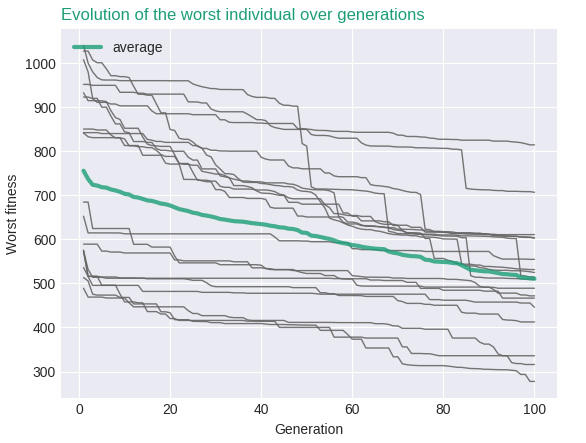
\includegraphics[scale=0.55]{exp1_worstIndv.png}
	\caption{In grey, different executions of the first experiment (E1)}\label{f:grahp1}
\end{figure}

Most executions from the previous experiment reached the maximum number of 
generations without stabilizing or converging. This means the EA may need a 
larger number of generations to fully evolve a solution. This is the hypothesis 
for the second experiment, which we describe next.

\subsection{Changing termination conditions}

% Antonio - You must introduce the experiment (each of them), trying to justify its necessity.

The main change in this implementation is the addition of two new stop conditions: being 10 generations without changes (stable population) or best fitness value below 0.01. 
% This should not be "also", it's maybe the most important change - JJ
% Antonio - I have stressed it. ;)
The set of operators is the same as the previous one, and the parameters remain 
unchanged except for the \textit{Number of generations} which is equal to 1000. 
The increase in the number of generations allows each run to fully develop 
their individuals. This would not be feasible if we had to simulate all the 
individuals, but thanks to the fitness function and the new stop conditions we 
can afford this number of generations.
% Antonio - why did you increase the number of generations? Explain it.
% Enphasize that we can run 1000 generations because fitness is
% designed to not having to use the simulator - JJ
% Updated - Laura

Although the best levels obtained with this experiment are better than those 
evolved in the first experiment, the bad solutions have a really high fitness 
value. In table \ref{t:resOver}, we can see that average fitness of levels 
produced with this version of the EA is worse than the ones generated in the 
first experiment. It suggest that populations can be stuck for many generations 
before making any type of improvement. Any of the generated levels have a 
fitness below 0.01 or reached maximum number of generations, which means the 
termination criteria that stopped the evolution was that the population was 
stable, without any new individuals added for 10 generations. 
\begin{figure}[H]
	\centering
	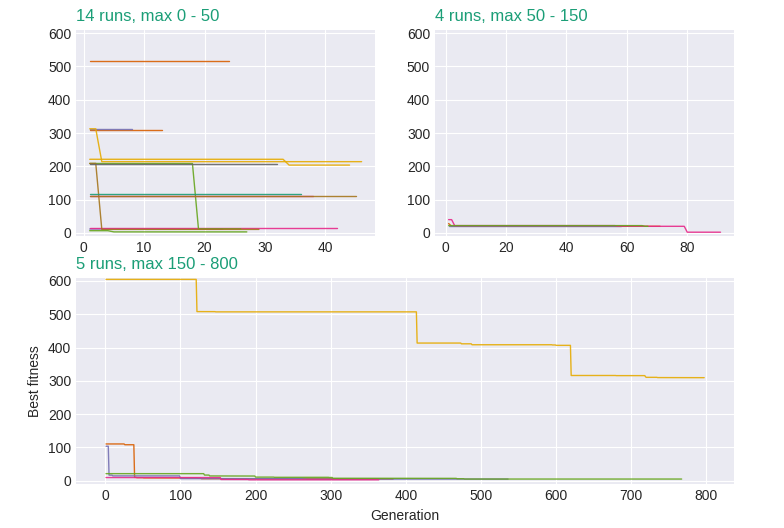
\includegraphics[scale=0.5]{exp2_explication.png}
	\caption{Best individual evolution for all executions, grouped by number of 
	generations}\label{f:grahp2}
\end{figure}
Figure \ref{f:grahp2} represents the evolution of the best individual of each 
execution. Most of them have no more than 50 generations, therefore the 
hypothesis for this experiment is not correct. Short evolutions show that the 
best individual at initialization is very similar to the last one. Slight 
improvements may be achieved by small mutations but it seems difficult for new 
generations to outperform previous ones. We can appreciate that significant 
improvements are most common in those executions with a poor initial 
population. Even the ones with several hundreds of generations struggle to 
improve the initial population.

Our hypothesis that the number of generations could be the main factor
is then not correct; it is more likely that there this EA is biased towards 
exploration rather than exploitation. The genetic operators are failing to 
create new individuals that inherit good traits from their parents. A new 
crossover operator could shift the focus to exploitation, and we will
examine this in the next experiment.

\subsection{Improving exploitation by a better crossover operator}


For the third experiment, the change introduced is in the crossover operator 
used which was previously described as \textit{Common blocks} crossover. 
The rest of the operators as 
well as the termination criteria are kept the same. 


Table \ref{t:resOver} shows that the results have radically improved as the 
average fitness of the best solutions drops to $0.0015$, a decrease of almost 
100\%. Additionally, it took less generations in general to reach those 
results. However, executions took longer on average, which makes sense given 
that a greater number of individuals would have been simulated. The average 
fitness of the population and the worst individual have similar values now, 
which suggest that in most executions the population did converge.

The levels are stable and the blocks do not fall when loading the level, but 
it is arguable that they would be be considered structures, since most of them consist in a 
few blocks spread about on the floor. The average amount of blocks is $6.26$, 
which is really close to the minimum amount of blocks allowed. However, given 
the proposed fitness function, it is completely logical that the evolution 
leads to this kind of arrangements. The more objects placed on the level, the 
more likely the individual is to not meet the requirements imposed by the 
constraints. It also makes sense to place objects near the ground, instead of 
one on top of the other.

The fitness landscape a fitness function creates is difficult to
assess, but in this case it is clear that search goes on the direction
of minimizing the number of blocks so that the number of blocks
actually falling is zero. The created structures are not very
interesting, though, that is why we propose some changes in the next experiment.

\subsection{Changing the minimum number of blocks per individual}

The only parameter that was changed for this experiment is the minimum
number, which went from 5 to 10. 

The first thing to notice in these experiments (Table \ref{t:resOver}) is the 
increase of the average execution time: it went from 1.76 hours in the third 
experiment to 5.03 hours in this one. The time spent running the simulation for 
each population in this experiments and in the previous one should be similar. 
However, the number of actual executions of the simulator, which only
kick in if there is actually some block on the floor and there is no overlap, drastically increased too. There is no doubt 
that placing at least ten objects in a structure that does not
collapse is more difficult than placing just five. The average 
best fitness value increased slightly, while the average and worst values are lower. This suggest that the latest generations of this EA are less diverse than those 
from the third experiment.

However, the results are more interesting visually. We can find some blocks 
being stack together, not only lied on the ground like in the previous 
experiment. 
% Comment on the actual appearance of these structures. Do they
% achieve the stated objective - JJ?
% I did change that - Laura

%************************************************



%%%%%%%%%%%%%%%%%%%%%%%%%%%%%  CONCLUSIONS  %%%%%%%%%%%%%%%%%%%%%%%%%%%%
%
\section{Conclusions and Future Work} 
\label{sec:conclusions}

% ----- probably should be eliminated --- 
% Here, we briefly recap several aspects of the development of this project. 
% First, we reviewed the context of the problem: PCG. In section 
%\ref{sec:intro}, 
% we looked at the main reasons for its existence: from replacing human 
% creativity where it cannot reach (unlimited or personalized) to enhancing and 
% speeding the creative process. In some cases, PCG can  be considered a kind 
%of 
% creative expression for itself. The technical background to approach the 
% problem is discussed in section \ref{sec:soa}.
% --- up to here --

This paper was developed with the main objective of implementing a
competitive entry for the Angry Birds level generation contest, and  a
set of sub-objectives in mind: exploring the expressiveness and variability of 
SBPCG with evolutionary techniques, adapting the game to extract data from 
execution and producing stable structures under gravity.
% What the intro to the conclusion should say are the main objectives
% of this paper, and whether they have been, or not, achieved or to
% what extent - JJ

% Antonio - This is my Proposal for this paragraph
For this aim we have implemented an Evolutionary Algorithm able to optimize 
level structures to meet some criteria, being the main one the stability of the 
constructions.
%Perhaps the level of achievement of the first objective, exploring the 
%expressiveness and variability of 
%SBPCG with evolutionary techniques,
%is not as easily measurable as the other two. It could seem like
%this objective has not been fully accomplished: only one SBPCG method
%has been implemented and tested. However, it was not in the scope of
%this work to test SBPCG in general, but in this particular case, for
%this particular game.
Considering this, the method studied was
sufficiently general and flexible to draw some conclusions about the
topic. SBPCG methods are a potential good solution to offline content
generation but it requires a great amount of problem-specific
knowledge. Like any other form of creative work, the biggest issue may
be how to measure how good, creative or enjoyable is the piece. The
more rules the author adds, expressiveness starts to get lost as the
results are variations of the same idea. However, it is crystal clear
from the experiments run in this paper that a lack of knowledge
will lead to unexpected outcomes.
In our case, the fitness function used the 
stability of the structure and only considered other features--- overlapping 
blocks and distance to the ground--- to ensure the levels would be valid.

 % I am lost in this paragraph. It should be more
 % related to the actual experiments made - JJ

The second objective, adapting the game to extract data from execution, was 
certainly achieved. It was also a basic requirement to proceed with the rest of 
them. The game does provide the data, as long as the input is correctly 
structured. 
% Although the original intention was to make it available on Linux, 
% currently it can only be executed with the desired behaviour on Windows. 
% Antonio - I think this is not relevant
% Another issue is that the simulation is not easily adaptable. If the fitness 
% function of the EA is changed and needs data that is not included in the 
%output 
% right now, the game would have to be changed and compiled again. 
% Antonio - I would suggest this text instead
In order to conduct our experiments the Angry Birds simulator (Science Birds) 
has been adapted to our necessities, yielding now some  other information 
required to evaluate the individuals of the implemented EA.
It would be interesting to obtain other kind of data from the simulator,
such as the height of the structure and, eventually, its resistance to
bombardment by angry birds. However, this is left as future work.

Producing stable structures under gravity was the third objective and
the closest to the ultimate one. That objective was effectively
achieved, but the consequence of evolving in a path of minimum
movement or maximum stability results in structures that are close to
the ground and do not have more than a few floors , which could not be very 
exciting for the players. 
% Antonio - I would add:
% , which could not be very exciting for the players. 
% Tell me what you think of this.
% Floors is not precise. ..more than a few stacked blocks? - Mario 
The main issue is, then, how we evaluate the levels. In fact this is 
a matter of how we define what an Angry Birds' level \textit{is} and if that 
definition matches the fitness function.
%A lot of elements were correct, but the definition was not complete.
How this definition of level plays
with the paths of evolution is also a problem. Since we define as
level as a structure that is stable, evolution will maximize stability
finding, as in the beginnings of architectural practice, squat
structures that are neither aesthetically pleasing nor playable,
although undeniably sturdy and stable. We have been successful in,
evolving free form structures, to find these type. But once we get
there, we need to go into a different evolution mode that takes into
account several features as a multiobjective optimization problem:
stability is the first, but we can sacrifice a bit of stability for
height or some other aesthetic quality.

% This idea brings us to the last objective, that was not achieved. Without 
% results that match the definition of an Angry Birds level, placing the 
% remaining objects would not have made the level playable. The partial 
% achievement of the third goal, blocked the fourth one as this objective was 
% dependent on the third one.

To conclude on an optimistic tone, this work provides an interesting insight 
into the SBPCG, through the completion---and failure---of the goals we
set out to achieve at the beginning.

In order to improve the results of the method, different constraints could be 
expressed as multiple objectives. Overlapping blocks and velocity could 
be treated as minimization objectives and height as a maximization one. % but 
%of course we don't need
                                % to minimize height any more... - JJ
                                % Corrected - Laura

If we pay attention at the stages of evolution in this work, there is also 
room for improvement in the genetic operators. For example, the initialization 
produces a small amount of valid individuals which suggested that an elitist 
strategy for selection would work best. However, new experiments will help to 
better balance exploration and exploitation. An interesting addition
would be to add {\em building} operators that pile blocks on
structures that are already stable. % Check out this idea, Laura - JJ
 % I like it, let's keep it - Laura

% First a discussion to say if the goal can be achieved using these
% methods. That is, finding stable structures is just a matter of
% adding more to the minimum numbre of blocks or more generations? - JJ

% ---- If we need 5 hours for every run, this is not realistic --- 
% Once we had a generator that meets our expectations, performance could be 
% enhanced by the analysis of the best set of initial parameters using Analysis 
% of Variance (or ANOVA), as presented in \cite{estevez2017statistical}. 

% ---- Some kind of "building" could be combined as genetic operator,
% but that would create structures that are too similar -- JJ
% -------------
% Some options were discarded for time limitations, so these could be main areas 
% of development. The chromosome representation using generative grammatical 
% encoding\cite{hornby2001advantages}, although it would radically change the 
% structure of the method, might ensure that generated levels are consistent. 
% This would require carefully selection the operators that would be the building 
% blocks of the generative grammar.


Another important issue that needs to be addressed is the time performance. 
Right now the simulation is the main bottleneck in the execution. One way to 
speed up the process can be \textit{cleaning} up the current simulation, getting 
rid of any unnecessary assets while maintaining the bare minimum to
perform evaluation. 
%However, this will not solve the problem, since the content generator will still need to launch an external executable.
% Antonio - I would not mention future problems

The communication between the simulation and the content generator is through 
read and write operations on disk, instead of memory. This could be avoided if 
both tools were integrated in one. If we aim for an online automatic generator, 
the generator should be integrated in the game. However, if our goal is to 
generate levels for mixed authorship, as an assistance to developers, it may be 
a better idea to integrate the simulation in the generator. This could be done 
by approximating in-game physics with real physics, as described in 
\cite{blum1970stability}. % Expand on this - JJ
% Or maybe eliminate if there's no space - JJ


%************************************************

\section*{Acknowledgements}
% This paper has been supported in part by
% \href{http://geneura.wordpress.com}{GeNeura Team}, 
% projects TIN2014-56494-C4-3-P (Spanish Ministry of Economy and
% Competitiveness) and DeepBio (TIN2017-85727-C4-2-P).
Acks taking\\
this much space.

\bibliographystyle{splncs03}
\bibliography{angrybirds}



\end{document}
